\documentclass{article}
\usepackage{amsmath, amsthm, amssymb, amsfonts}
\usepackage{thmtools}
\usepackage{graphicx}
\usepackage{setspace}
\usepackage{geometry}
\usepackage{float}
\usepackage{hyperref}
\usepackage[utf8]{inputenc}
\usepackage[english, spanish]{babel}
\usepackage{framed}
\usepackage[dvipsnames]{xcolor}
\usepackage{tcolorbox}
\usepackage{pgfplots}
\usepackage{tikz}
\usetikzlibrary{arrows, positioning}
\usepackage{bbm}
\pgfplotsset{compat=1.18}

\colorlet{LightGray}{White!90!Periwinkle}
\colorlet{LightOrange}{Orange!15}
\colorlet{LightGreen}{Green!15}

\newcommand{\HRule}[1]{\rule{\linewidth}{#1}}

\declaretheoremstyle[name=Teorema,]{thmsty}
\declaretheorem[style=thmsty,numberwithin=section]{theorem}
\tcolorboxenvironment{theorem}{colback=LightGray}

\declaretheoremstyle[name=Ejercicio,]{prosty}
\declaretheorem[style=prosty,numberlike=theorem]{exercise}
\tcolorboxenvironment{exercise}{colback=LightOrange}

\declaretheoremstyle[name=Demostración,]{prcpsty}
\declaretheorem[style=prcpsty,numberlike=theorem]{proofs}
\tcolorboxenvironment{proofs}{colback=LightGreen}

\declaretheoremstyle[name={..}, numbered=no,]{prcpsty_nonum}
\declaretheorem[style=prcpsty_nonum,unnumbered]{proofs*} % Unnumbered version
\tcolorboxenvironment{proofs*}{colback=LightGreen}

\setstretch{1.2}
\geometry{
    textheight=9in,
    textwidth=5.5in,
    top=1in,
    headheight=12pt,
    headsep=25pt,
    footskip=30pt
}


% -------------------------------------------------------------------
% Comando para crear portadas internas de temas
% -------------------------------------------------------------------
\newcommand{\temaportada}[1]{
    \newpage
    \refstepcounter{section} % Incrementa el contador de sección (para numeración)
    \addcontentsline{toc}{section}{#1} % Añade al índice sin número visible

    \begin{center}
        \vspace*{2cm}
        \HRule{1.2pt} \\[0.4cm]
        {\LARGE \bfseries #1 \\[0.4cm]}
        \HRule{1.2pt} \\[2cm]
        {\large \textit{Procesos Estocásticos}}\\[1.5cm]
        {\normalsize Universidad de Valladolid}\\[0.5cm]
        {\normalsize \today}
        \vfill
    \end{center}
    \newpage
}

% ------------------------------------------------------------------------------

\begin{document}

% ------------------------------------------------------------------------------
% Cover Page and ToC
% ------------------------------------------------------------------------------

\title{ \normalsize \textsc{}
\\ [2.0cm]
\HRule{1.5pt} \\
\LARGE \textbf{\uppercase{Ejercicios Procesos Estocásticos}
}
}
\author{\textbf{Author} \\
    Victor Elvira Fernández, Tomás Ruiz Rojo,\\ Juan Horrillo Crespo, Irene Retortillo González \\
    Universidad de Valladolid \\
    \date{\today}}

\maketitle
\newpage

\include{colaboraciones}

\tableofcontents
\newpage

% ------------------------------------------------------------------------------
\temaportada{Tema 1: Cadenas de Markov en Tiempo Discreto}
\subsection{Parte 1}
\subsubsection{Ejercicio 1}
\begin{exercise}
Una moneda justa se lanza de forma reiterada, con resultados $Y_0, Y_1, Y_2, \ldots$ 
(identificamos \emph{cara} con $1$ y \emph{cruz} con $0$).  

Para cada $n \geq 1$, se define
\[
X_n = Y_n + Y_{n-1}
\]
como el número de caras obtenidas en los lanzamientos $n-1$ y $n$.  

¿Es $X_n$ una cadena de Markov? En caso afirmativo, describe la matriz de transición.
\end{exercise}

Suponemos un espacio E=$\{0,1,2\}$. Para que sea cadena de Markov, $X_n$ deberá depender de n y no de los estados anteriores.
\[
P\left(X_{n+1}/ X_n, X_{n-1},\dots, X_0\right) = P\left(X_{n+1}/ X_n\right)
\]

Esto a simple vista podemos ver que \textbf{no es una cadena de Markov}

¿Por qué?. Lo demostramos con un ejemplo.

\[
P \left(X_3 = 0 / X_2 =1, X_1=0\right) = 0 \rightarrow P \left( X_2 =1,X_1=0\right) = P(Y_0=0,Y_1=0,Y_2=1)
\]
$X_3$ no podrá ser en este caso 0 y por eso la probabilidad es 0.

En cambio:
\[
P\left(X_3=0 / X_2=1, X_1=2\right) = P \left( X_3 =0 / Y_0 = 1,Y_1 =1, Y_2=0\right) = \frac{1}{2}
\]

Si fuera una cadena de Markov $P(X_3=0)$ debería ser igual en ambos casos. Por lo tanto concluimos que depende $X_n$ depende de los estados anteriores y no es una cadena de Markov.

\subsubsection{Ejercicio 2}
\begin{exercise}
Un conductor de taxi se mueve entre el aeropuerto $A$ y dos hoteles, $B$ y $C$, de acuerdo con las siguientes reglas:

\begin{itemize}
    \item Si está en el aeropuerto, después estará en uno de los dos hoteles con igual probabilidad.
    \item Si está en un hotel, volverá al aeropuerto con probabilidad $\frac{3}{4}$ o irá al otro hotel con probabilidad $\frac{1}{4}$.
\end{itemize}

\begin{enumerate}
    \item Escribe la matriz de transición de la cadena de Markov.
    \item Supongamos que el conductor está en el aeropuerto en el tiempo $n=0$. Calcula la probabilidad de estar en cada una de las tres localizaciones posibles en $n=2$ y la probabilidad de que esté en un hotel en $n=3$.
\end{enumerate}
\end{exercise}


Partiendo del espacio de estados: $E=\{A,B,C\}$ donde A es el aeropuerto y B y C son los dos hoteles.

Vemos que este problema viene dado por una Cadena de Markov, ya que el estado es independiente de n y solo depende del estado anterior.

Se nos pide la matriz de transición de la cadena. Observando el enunciado vemos que la matriz de transición es:

\[
\mathbb{P} =
\begin{pmatrix}
    0 & \frac{1}{2} & \frac{1}{2}\\
    \frac{3}{4} & 0 & \frac{1}{4} \\
    \frac{3}{4} & \frac{1}{4} & 0\\
\end{pmatrix}
\]

Se nos pide calcular la probabilidad de que esté en cualquiera de las 3 localizaciones en n=2, sabiendo que está en el aeropuerto (A) en n=0.
Es decir:
\[
P(X_2=A \mid X_0=A) \quad P(X_2=B \mid X_0=A) \quad P(X_2=C \mid X_0=A)
\]

Lo podemos calcular de manera manual o a través de la matriz de transiciones. Lo calcularemos de ambas formas para ilustrar que el resultado es el mismo:
\[
P(X_2=A\mid X_0=A)=\sum_{s\in\{A,B,C\}} P(X_1=s\mid X_0=A)P(X_2=A\mid X_1=s)
=0\cdot0+\tfrac12\cdot\tfrac34+\tfrac12\cdot\tfrac34=\tfrac34,
\]

Aunque se pueda calcular así, es mucho más sencillo usando la matriz de transición.

\[
\mathbb{P}^2 = \mathbb{P} \cdot \mathbb{P} = 
\begin{pmatrix}
    0 & \frac{1}{2} & \frac{1}{2}\\
    \frac{3}{4} & 0 & \frac{1}{4} \\
    \frac{3}{4} & \frac{1}{4} & 0\\
\end{pmatrix}
\cdot
\begin{pmatrix}
    0 & \frac{1}{2} & \frac{1}{2}\\
    \frac{3}{4} & 0 & \frac{1}{4} \\
    \frac{3}{4} & \frac{1}{4} & 0\\
\end{pmatrix}
=
\begin{pmatrix}
    \frac{3}{4} & \frac{1}{8} & \frac{1}{8} \\
    \frac{3}{16} & \frac{3}{8} & \frac{5}{16} \\
    \frac{3}{16} & \frac{5}{16} & \frac{3}{8} \\
\end{pmatrix}
\]

Como nos interesa para $X_0=A$, nos quedamos con la primera fila y vemos que las probabilidades son $\left(\frac{3}{4}, \frac{1}{8}, \frac{1}{8}\right)$

\subsubsection{Ejercicio 5}


\begin{exercise}
Sea $\{X_n\}_{n\ge 0}$ una cadena de Markov homogénea con espacio de estados $E$ y matriz de transición $P$.  
Sea $\tau$ el primer instante para el que $X_n \neq X_0$, donde $\tau = \infty$ si $X_n = X_0$ para todo $n \ge 0$.  

Calcula $\mathbb{E}[\tau \mid X_0 = i]$ en términos de $p_{ii}$.
\end{exercise}
\[
\tau \in \{1,2,3\} \cup \{\infty\}.
\]
Si $\tau=4 \Rightarrow$ (por ejemplo) $x_0=0, x_1=0, x_2=0, x_3=0, x_4=1$, ya que $x_n \neq x_0$.

La probabilidad de que $\tau=\infty$ es 0:
\[
P(\tau=\infty \mid X_0=i) = \lim_{n \to \infty} P(\tau > n \mid X_0=i) = \lim_{n \to \infty} p_{ii}^{n} = 0.
\]

Ahora calculamos la esperanza:
\[
P(\tau=1\mid X_0=i)=1-p_{ii}, \quad 
P(\tau=2\mid X_0=i)=p_{ii} \cdot (1-p_{ii}), \quad \dots
\]
\[
P(\tau=n \mid X_0=i)=p_{ii}^{\,n-1} \cdot (1-p_{ii})
\]

Por lo tanto:
\[
E(\tau \mid X_0=i) = \sum_{k=1}^{\infty} k \cdot P(\tau=k \mid X_0=i) = (1-p_{ii}) \sum_{k=1}^{\infty} k \cdot p_{ii}^{\,k-1} = \frac{1}{1-p_{ii}}.
\]

Vemos que $\tau$ sigue una distribución geométrica de parámetro $1-p_{ii}$:
\[
\tau \sim \text{Geom}(1-p_{ii}).
\]


\subsubsection{Ejercicio 7}
\begin{exercise}
Sea $\{Z_n\}_{n \geq 1}$ una sucesión de variables aleatorias independientes e idénticamente distribuidas (v.a.i.i.d.) geométricas, es decir, tales que, para $k \geq 0$,
\[
P(Z_n = k) = (1 - p)^k p, \quad \text{con } p \in (0,1).
\]
Sea $X_n = \max(Z_1, \dots, Z_n)$. 

Demuestra que $\{X_n\}_{n \geq 1}$ es una cadena de Markov homogénea y da su matriz de transición.
\end{exercise}

Primero comprobamos que $\{X_n\}_{n\geq 1}$ es una cadena de Markov. Sabemos que $X_n = max(Z_1, \dots, Z_n)$. Para que sea una cadena de Markov $X_{n+1}$ solo podrá depender de $Z_{n+1}$ y del estado anterior $X_n$ (esto se puede aplicar porque $Z_n$ es v.a.i.i.d. y $Z_{n+1}$ no depende de $Z_n$).

Si calculamos $X_{n+1}$ vemos que:
\[
X_{n+1}=max(Z_1,\dots,Z_{n+1})=max(max(Z_1,\dots,Z_n),Z_{n+1})
\]
\[
X_{n+1}=max(X_n,Z_{n+1})
\]
Como solo depende del estado anterior y del valor de $Z_{n+1}$, $\{X_n\}_{n\geq 1}$ es una cadena de Markov.

Ahora calcularemos la matriz de transición.

Observando las condiciones vemos que el i,j-ésimo elemento de la matriz será:

\[
p_{ij}=
\left\{
\begin{matrix}
    0  \\
    \sum_{k=0}^{i} p \cdot (1+p)^k \\
    (1-p)^j \cdot p
\end{matrix}
\right.
\begin{matrix}
    j < i \\
    j = i \\
    j > i
\end{matrix}
\]
Esto ocurre porque si j<i el máximo no puede disminuir, entonces la probabilidad de pasar a un estado menor es 0.
Si j=i, el proceso se mantiene en el mismo estado siempre que $Z_{n+1} \leq i$ lo cual tiene una probabilidad de ocurrencia de: $P(Z_{n+1}=i)=1-(1-p)^{i+1}$
Si j >i, el máximo aumenta a j si $Z_{n+1}=j$, lo que ocurre con probabilidad $p \cdot (1-p)^j$.

La matriz de transición queda así:
\[
\mathbb{P}=
\begin{pmatrix}
(1-p)^1 & p(1-p)^1 & p(1-p)^2 & \cdots & p(1-p)^{i-1} \\[1mm]
0 & (1-p)^2 & p(1-p)^2 & \cdots & p(1-p)^{i-1}\\[1mm]
0 & 0 & (1-p)^3 & \cdots & p(1-p)^{i-1}  \\[1mm]
\vdots & \vdots & \vdots & \ddots & \vdots \\[1mm]
0 & 0 & 0 & \cdots & (1-p)^i\\[1mm]

\end{pmatrix}
\]



\subsubsection{Ejercicio 8}

\begin{exercise}
Supongamos que la probabilidad de que llueva hoy es $0.3$ si ninguno de los dos últimos días fue lluvioso, pero es $0.6$ si hubo lluvia en al menos uno de los dos. Si clasificamos el tiempo en el día $n$ como $W_n \in \{L,S\}$ (lluvioso o seco):

\begin{enumerate}
    \item ¿Es $\{W_n\}$ una cadena de Markov?
    \item Definimos $X_n = (W_{n-1}, W_n)$. ¿Es $\{X_n\}$ una cadena de Markov?
    \item Determina la matriz de transición de $\{X_n\}$.
    \item Si no llovió el domingo ni el lunes, ¿cuál es la probabilidad de que llueva el miércoles?
\end{enumerate}
\end{exercise}

\textbf{$W_n$}

$W_n$ será una cadena de Markov si su estado siguiente no depende de los estados anteriores.

\[
P(W_{n+1}=L \mid W_{n}=S, W_{n-1}=S)=0.3,\qquad
P(W_{n+1}=L \mid W_{n}=L\ \text{o}\ W_{n-1}=L)=0.6
\]

Como depende de los dos estados anteriores, $W_n$ \textbf{no es una cadena de Markov}.

\medskip
\textbf{$X_n=(W_{n-1},W_n)$}

Espacio de estados $E=\{SS,SL,LS,LL\}$

\[
\mathbb{P}=
\begin{pmatrix}
0.7 & 0.3 & 0   & 0   \\
0   & 0   & 0.4 & 0.6 \\
0.4 & 0.6 & 0   & 0   \\
0   & 0   & 0.4 & 0.6
\end{pmatrix}
\]

Ahora $X_n$ sí es una cadena de Markov, pues el siguiente estado depende sólo del par actual.

\textbf{Lluvia el miercoles}

Estado inicial (domingo, lunes) $=SS$.  
Queremos la probabilidad de que el miércoles (dos días después) llueva, es decir, que $W_{n+2}=L$.  
Esto ocurre si el estado al cabo de dos pasos es $SL$ o $LL$.

Calculamos $\mathbb{P}^2$:

\[
\mathbb{P}^2=
\begin{pmatrix}
0.49 & 0.21 & 0.18 & 0.12\\
0.42 & 0.18 & 0.24 & 0.16\\
0.49 & 0.21 & 0.18 & 0.12\\
0.42 & 0.18 & 0.24 & 0.16
\end{pmatrix}
\]

Desde $SS$, las probabilidades a dos pasos son la primera fila: $(0.61,\,0.21,\,0.12,\,0.06)$.

La probabilidad de que el tercer día (miércoles) sea lluvioso es:
\[
P(W_{n+2}=L \mid SS)=P(X_{n+2}\in\{SL,LL\})=0.49+0.18=0.67.
\]


\subsubsection{Ejercicio 9}
\begin{exercise}
Sea $\{X_n\}_{n\ge0}$ una cadena de Markov homogénea con espacio de estados $E$ y matriz de transición $P=(p_{ij})_{i,j\in E}$. Para $L\ge1$ definimos
\[
Y_n=(X_n,X_{n+1},\dots,X_{n+L}).
\]
El proceso $\{Y_n\}_{n\ge0}$ toma valores en
\[
F=\{(i_0,i_1,\dots,i_L)\in E^{L+1}:\; p_{i_0 i_1}p_{i_1 i_2}\cdots p_{i_{L-1} i_L}>0\}.
\]
Demuestra que $\{Y_n\}$ es una cadena de Markov homogénea y da su matriz de transición (cadena serpiente de orden $L$).
\end{exercise}

Queremos probar que
\[
P(Y_{n+1}=\vec{j} \mid Y_n=\vec{i}, Y_{n-1}=\vec{v},\dots,Y_0=\vec{v_0})
= P(Y_{n+1}=\vec{j} \mid Y_n=\vec{i}).
\]

Sabiendo que
\[
\vec{j}=(j_0,j_1,\dots,j_L), \qquad \vec{i}=(i_0,i_1,\dots,i_L),
\]
tenemos que
\[
Y_{n+1}=(X_{n+1},X_{n+2},\dots,X_{n+L+1}).
\]
Entonces, para que la transición $\vec{i}\to\vec{j}$ sea posible, debe cumplirse
\[
j_0=i_1,\ j_1=i_2,\ \dots,\ j_{L-1}=i_L,
\]
y sólo la última coordenada cambia.

Por tanto:
\[
P(Y_{n+1}=\vec{j} \mid Y_n=\vec{i})
= P(X_{n+L+1}=j_L \mid X_{n+L}=i_L)
= p_{i_L j_L}.
\]
Si no se cumple la condición de solapamiento ($j_k=i_{k+1}$ para $k=0,\dots,L-1$), entonces la probabilidad es 0.

En resumen:
\[
P(Y_{n+1}=\vec{j}\mid Y_n=\vec{i})=
\begin{cases}
p_{i_L j_L}, & \text{si } (j_0,\dots,j_{L-1})=(i_1,\dots,i_L),\\[4pt]
0, & \text{en otro caso.}
\end{cases}
\]

Por tanto $\{Y_n\}$ es una cadena de Markov homogénea con matriz de transición $\mathbb{P}=(p_{\vec{i},\vec{j}})$ dada por
\[
p_{\vec{i},\vec{j}}=
\begin{cases}
p_{i_L j_L}, & \text{si } (j_0,\dots,j_{L-1})=(i_1,\dots,i_L),\\[4pt]
0, & \text{en otro caso.}
\end{cases}
\]

Esta construcción se denomina \textbf{cadena serpiente (snake chain)} de orden $L$ asociada a $\{X_n\}$.

\subsubsection{Ejercicio 11}

\begin{exercise}
Un ratón se mueve en un recinto con cinco parcelas, como se representa en el siguiente gráfico. 
El ratón parte del espacio 1. Cuando el ratón está en una parcela, elige cualquiera de las parcelas 
comunicadas con igual probabilidad, hasta que llega al espacio 3, donde está un gato, 
o al 5, donde hay un trozo de queso. 

\medskip
\noindent
¿Cuál es la probabilidad de que el ratón alcance el queso antes de ser comido por el gato?
\end{exercise}

\begin{figure}[H]
    \centering
    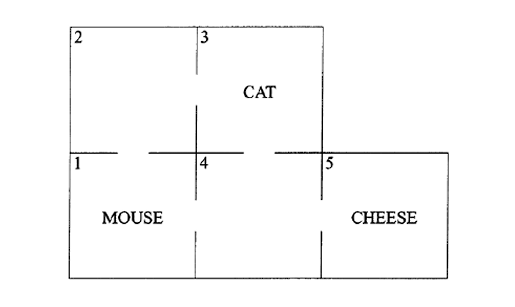
\includegraphics[width=0.6\textwidth]{tema1/img/ej11p1.png}
    \caption{Recinto con las cinco parcelas y posibles movimientos del ratón.}
    \label{ej11p1}
\end{figure}

Siendo $\tau_i$ el primer instante n tal que $X_n=i$:

\[
\tau_i = inf\{n \geq 0 : X_n=i\}
\]

Se nos pide hallar la probabidad de que el ratón alcance el queso. Planteamos las posibilidades llamando $\tau_5$ al queso y $\tau_3$ al gato
\[
\begin{matrix}
    P(\tau_5 < \tau_3 \mid X_0=1) = x \\
    P(\tau_5 < \tau_3 \mid X_0=2) = y \\
    P(\tau_5 < \tau_3 \mid X_0=3) = 0 \\
    P(\tau_5 < \tau_3 \mid X_0=4) = z \\
    P(\tau_5 < \tau_3 \mid X_0=5) = 1 
\end{matrix}
\]

Llamamos a las probabilidades de alcanzar el queso antes de ser comido x,y,z. Si la posición inicial es la 3 es claro que el gato ya nos habrá alcanzado y no podrremos alcanzar el queso antes observando la figura \ref{ej11p1}.
Ocurrirá lo mismo si la posición inicial es la 5, la probabilidad de alcanzar el queso será 1.

Resolveremos utilizando el método del primer paso que consiste en ir buscando ecuaciones recursivas basadas en lo que ocurre después del primer movimiento de la cadena.

Buscamos despejar x,y,z:
\[
\begin{matrix}
    x= P(\tau_5 < \tau_3 \mid X_0=1) = P(\tau_5 < \tau_3 , X_1=2 \mid X_0=1) + P(\tau_5 < \tau_3 , X_1=4 \mid X_0=1) \\
    x= \tfrac12 \cdot y + \tfrac12 \cdot z
\end{matrix}
\]

\[
\begin{matrix}
    y=P(\tau_5 < \tau_3 \mid X_0=2) = P(\tau_5 < \tau_3, X_1=1 \mid X_0=2)+P(\tau_5 < \tau_3, X_1=3 \mid X_0=2) \\
    y = \tfrac12 \cdot x + \tfrac12 \cdot 0 = \tfrac12 \cdot x
\end{matrix}
\]

\[
\begin{matrix}
    z=P(\tau_5 < \tau_3 \mid X_0=4) = P(\tau_5 < \tau_3, X_1=1 \mid X_0=4) + P(\tau_5 < \tau_3, X_1=3 \mid X_0=4)\\ + P(\tau_5 < \tau_3, X_1=5 \mid X_0=4) \\
    z= \tfrac13 \cdot x + \tfrac13 \cdot 1 \tfrac13 \cdot 0 = \tfrac13 \cdot x + \tfrac13 
\end{matrix}
\]

Planteamos el sistema de ecuaciones y resolvemos:
\[
\begin{matrix}
    x = \tfrac12 \cdot y + \tfrac12 \cdot z \\
    y = \tfrac12 \cdot x \\
    z= \tfrac13 \cdot x + \tfrac13 
\end{matrix}
\]
Resolvemos:
\[
\begin{matrix}
    x = \tfrac14 x + \tfrac16 x +\tfrac16 \Longrightarrow \frac{7}{12} \cdot x = \tfrac16 \Longrightarrow x = \frac{12}{7} \cdot \tfrac16 \\
    x = \tfrac27
\end{matrix}
\]
\medskip
\[
    y= \tfrac12 \cdot\tfrac27 = \tfrac17
\]
\medskip
\[
z=\tfrac13 \cdot \left(1 + \tfrac27\right) = \tfrac13 \cdot \tfrac97 = \tfrac37
\]    


\subsubsection{Ejercicio 15}
\subsubsection{Ejercicio 17}
\begin{exercise}
Prueba que el siguiente grafo de transición es irreducible. Calcula el periodo y las clases cíclicas.
\end{exercise}

Se nos da la secuencia de transiciones:
\[
1 \rightarrow 4 \rightarrow 3 \rightarrow 2 \rightarrow 7 \rightarrow 6 \rightarrow 1 \rightarrow 4 \rightarrow 5 \rightarrow 2 \rightarrow 7 \rightarrow 6 \rightarrow 2 \rightarrow 7 \rightarrow 6 \rightarrow 1 \dots
\]
(EL grafo tambien se nos da, consulta los enunciados amego)

El conjunto de estados es \(S=\{1,2,3,4,5,6,7\}\).

Para probar que la cadena es irreducible basta demostrar que todo par de estados se comunican. Observemos que desde cualquier estado se puede alcanzar el estado \(2\):
\[
1\to4\to3\to2,\quad 4\to3\to2,\quad 3\to2,\quad 5\to2,\quad 6\to2,\quad 7\to6\to2.
\]
Por otro lado, desde \(2\) se puede llegar a cualquier otro estado recorriendo el grafo:
\[
2\to7\to6\to1\to4\to3,\quad \text{y también } 4\to5.
\]
Por tanto, desde \(2\) se puede alcanzar a todos los demás estados. Dado que cualquier estado llega a \(2\) y \(2\) llega a cualquiera, se tiene que todos los estados se comunican entre sí. La cadena es, por tanto, \textbf{irreducible}.

Para el cálculo del periodo recordemos que
\[
A_i = \{n\ge1 : p_{ii}^{(n)} > 0\}, \quad d(i) = \gcd A_i.
\]
Como la cadena es irreducible, el periodo es el mismo para todos los estados, por lo que basta calcularlo para \(i=2\). Encontramos ciclos que comienzan y terminan en \(2\):
\[
2 \to 7 \to 6 \to 2 \quad (\text{longitud } 3), \qquad
2 \to 7 \to 6 \to 1 \to 4 \to 3 \to 2 \quad (\text{longitud } 6),
\]
y también concatenaciones de ellos de longitud \(9, 12, \dots\). El conjunto de longitudes posibles es, pues, \(\{3,6,9,\dots\}\), y su máximo común divisor es
\[
d(2) = \gcd\{3,6,9\} = 3.
\]
Luego el periodo de toda la cadena es \(3\).

Para determinar las clases cíclicas agrupamos los estados según la congruencia módulo \(3\) del número de pasos mínimos desde un estado de referencia (por ejemplo, desde \(1\)):
\[
\begin{array}{lcl}
\text{distancia 0 (mod 3):} & \{1,2\},\\
\text{distancia 1 (mod 3):} & \{4,7\},\\
\text{distancia 2 (mod 3):} & \{3,5,6\}.
\end{array}
\]
Estas son las tres clases cíclicas, y se observa que cada transición lleva de una clase a la siguiente, de modo que el patrón se repite cada tres pasos, consistente con el periodo \(3\).

En conclusión, el grafo es \textbf{irreducible}, tiene \textbf{periodo 3} y sus \textbf{clases cíclicas} son:
\[
\boxed{\mathbb{C}_0 = \{1,2\}, \quad \mathbb{C}_1 = \{4,7\}, \quad \mathbb{C}_2 = \{3,5,6\}.}
\]

\subsubsection{Ejercicio 19}
\subsubsection{Ejercicio 20}
\subsubsection{Ejercicio 21}
\subsubsection{Ejercicio 22}
\begin{exercise}
Prueba que la cadena del problema 7 no tiene distribución estacionaria.
\end{exercise}

Recordemos que en el \textbf{Ejercicio 7} se definía la sucesión $\{X_n\}_{n\ge1}$ como
\[
X_n = \max(Z_1, Z_2, \dots, Z_n),
\]
donde $\{Z_n\}_{n\ge1}$ son variables aleatorias independientes e idénticamente distribuidas, con distribución geométrica:
\[
\mathbb{P}(Z_n = k) = (1-p)^k p, \quad k = 0,1,2,\dots, \quad p \in (0,1).
\]

\paragraph{Recordatorio de la matriz de transición.}
Sabemos que $\{X_n\}$ es una cadena de Markov homogénea con matriz de transición
\[
P_{i,j} = 
\begin{cases}
0, & j < i,\\[4pt]
1-(1-p)^{i+1}, & j = i,\\[4pt]
(1-p)^j p, & j > i.
\end{cases}
\]
Esto se debe a que
\[
X_{n+1} = \max(X_n, Z_{n+1}),
\]
por lo que dado $X_n = i$, el siguiente estado depende únicamente del nuevo valor $Z_{n+1}$.

\paragraph{Comprobación de la posible distribución estacionaria.}
Sea $\pi = (\pi_0, \pi_1, \pi_2, \dots)$ una distribución estacionaria, es decir:
\[
\pi = \pi P, \quad \text{con} \quad \sum_{k=0}^\infty \pi_k = 1.
\]
De la primera ecuación:
\[
\pi_0 = p \cdot \pi_0 \quad \Longrightarrow \quad \pi_0(1-p) = 0 \quad \Longrightarrow \quad \pi_0 = 0.
\]
Para el siguiente estado:
\[
\pi_1 = (1-p)p \pi_0 + \left[p + (1-p)p\right] \pi_1 + \sum_{j>1}(1-p)^j p \pi_j.
\]
Como $\pi_0 = 0$, y todos los coeficientes multiplicativos son menores que 1, se obtiene inductivamente que todas las probabilidades $\pi_k$ deben ser nulas:
\[
\pi_k = 0 \quad \text{para todo } k \ge 0.
\]
Por tanto, el único vector que satisface $\pi = \pi P$ es el vector nulo, el cual no es una distribución de probabilidad.

Por tanto, la cadena $X_n$ no tiene distribución estacionaria.
\subsubsection{Ejercicio 23}
\begin{exercise}
Supongamos que $\{X_n\}_{n\ge0}$ es un proceso de ramificación (branching process), de forma que $X_n$ representa el tamaño de la generación $n$. Asumimos que la generación inicial está formada por un solo individuo y que la distribución del número de descendientes de uno de estos individuos tiene media $\mu$ y varianza $\sigma^2$. Demuestra que el tamaño medio de la generación $n$ satisface la relación de recurrencia
\[
\mathbb{E}X_{n+1}=\mu\,\mathbb{E}X_n,\qquad n\ge0,
\]
y concluye que $\mathbb{E}X_n=\mu^n,\ n\ge1$. Demuestra también que la varianza satisface
\[
\operatorname{Var}(X_{n+1})=\mu^2\operatorname{Var}(X_n)+\sigma^2\mu^n,\qquad n\ge0,
\]
y comprueba, a partir de esta relación, que
\[
\operatorname{Var}(X_n)=
\begin{cases}
n\sigma^2, & \mu=1,\\[6pt]
\sigma^2\,\dfrac{\mu^{n-1}(\mu^n-1)}{\mu-1}, & \mu\neq1,
\end{cases}\qquad n\ge1.
\]
(Indicación: para obtener las recurrencias estudia la esperanza o la varianza de $X_{n+1}$ condicionada por $X_n$.)
\end{exercise}


Por definición del proceso de ramificación,
\[
X_{n+1}=\sum_{j=1}^{X_n} Z_n^{(j)},
\]
donde $\{Z_n^{(j)}\}$ son iid con media $\mu$ y varianza $\sigma^2$, y para cada $n$ los $Z_n^{(j)}$ son independientes de $X_n$.

Condicionando por $X_n$ obtenemos la esperanza condicional
\[
\mathbb{E}(X_{n+1}\mid X_n=k)=\mathbb{E}\Big(\sum_{j=1}^k Z_n^{(j)}\Big)=k\mu,
\]
luego
\[
\mathbb{E}(X_{n+1}\mid X_n)=\mu X_n.
\]
Tomando esperanza en ambos lados (ley de la esperanza total)
\[
\mathbb{E}X_{n+1}=\mathbb{E}\big(\mathbb{E}(X_{n+1}\mid X_n)\big)=\mathbb{E}(\mu X_n)=\mu\,\mathbb{E}X_n.
\]
Con $X_0=1$ se obtiene por recurrencia $\mathbb{E}X_n=\mu^n$ para $n\ge1$.

Para la varianza usamos la descomposición de la varianza condicionada:
\[
\operatorname{Var}(X_{n+1})=\mathbb{E}\big(\operatorname{Var}(X_{n+1}\mid X_n)\big)+\operatorname{Var}\big(\mathbb{E}(X_{n+1}\mid X_n)\big).
\]
Dado $X_n=k$, la suma de $k$ variables iid tiene varianza $k\sigma^2$, luego
\[
\operatorname{Var}(X_{n+1}\mid X_n=k)=k\sigma^2 \quad \operatorname{Var}(X_{n+1}\mid X_n)=X_n\sigma^2.,
\]
y por tanto (ley de la esperanza)
\[
\mathbb{E}\big(\operatorname{Var}(X_{n+1}\mid X_n)\big)=\mathbb{E}(X_n\sigma^2)=\sigma^2\mathbb{E}X_n=\sigma^2\mu^n.
\]
Además
\[
\operatorname{Var}\big(\mathbb{E}(X_{n+1}\mid X_n)\big)=\operatorname{Var}(\mu X_n)=\mu^2\operatorname{Var}(X_n).
\]
Por tanto se obtiene la recurrencia para la varianza:
\[
\operatorname{Var}(X_{n+1})=\mu^2\operatorname{Var}(X_n)+\sigma^2\mu^n,\qquad n\ge0,
\]
con condición inicial $\operatorname{Var}(X_0)=0$.

Resolvemos esta recurrencia. Sea $v_n=\operatorname{Var}(X_n)$. Entonces
\[
v_{n+1}=\mu^2 v_n+\sigma^2\mu^n,\qquad v_0=0.
\]
Iterando la relación se obtiene la suma telescópica
\[
v_n=\sigma^2\sum_{k=0}^{n-1}\mu^{\,n-1+k}=\sigma^2\mu^{\,n-1}\sum_{k=0}^{n-1}\mu^{k}
=\sigma^2\mu^{\,n-1}\frac{\mu^{n}-1}{\mu-1},\qquad (\mu\neq1).
\]
En el caso $\mu=1$ tomamos límite (o bien observamos la recurrencia \(v_{n+1}=v_n+\sigma^2\) con \(v_0=0\)) y obtenemos
\[
v_n=n\sigma^2,\qquad (\mu=1).
\]
En resumen,
\[
\operatorname{Var}(X_n)=
\begin{cases}
n\sigma^2, & \mu=1,\\[6pt]
\sigma^2\,\dfrac{\mu^{n-1}(\mu^n-1)}{\mu-1}, & \mu\neq1,
\end{cases}\qquad n\ge1,
\]
como pedía el enunciado.






s
% \include{src/clase1212}

% \include{src/Clase1320}
% \include{src/clase2012}

\newpage

% ------------------------------------------------------------------------------
% Reference and Cited Works
% ------------------------------------------------------------------------------

\begin{thebibliography}{9}
    \bibitem{diapos1}
    Inés Velasco, \\ \textit{Ejercicios Manuscritos}. \\ Universidad de Valladolid 2025.
\end{thebibliography}

% ------------------------------------------------------------------------------

\end{document}
